\section{Database}
\subsection{Introduzione}
Questa sezione tratterà la gestione del database dell'applicazione BlockCovid. Nel sistema implementato da DPCM2077, il database è direttamente collegato al backend.

\subsubsection{Scopo}
Il database permette al backend di memorizzare i dati che servono per il corretto funzionamento dell'applicazione. Essendo il database implementato nel backend, questa sezione è dedicata a chi gestisce il database e sviluppa il backend.

\subsection{Requisiti e installazione}
Per poter aggiungere funzionalità al database del sistema BlocKCovid, sono necessari gli strumenti indicati in questa sezione. Per semplicità è consigliato l'utilizzo di docker per l'esecuzione del servizio.

\subsubsection{Prerequisiti hardware e software}
È consigliato l'utilizzo di un server con risorse sufficienti per il funzionamento del database. Questo dipende molto dalla quantità dei dati e per questo è consigliato avere risorse hardware equivalenti ad un processore quad-core e 8 GB di RAM e sufficiente spazio su disco.
\\\\
Il database di riferimento è MariaDB 10.5.9.

\subsubsection{Ottenimento script}
Per scaricare gli script necessari alla creazione e popolamento database è necessario \textbf{Git}. Se non si dispone di Git è possibile scaricarlo seguendo quanto indicato nella sezione \textbf{§4.2.4}. Per scaricare il progetto, invocare il seguente comando da terminale: \textit{git clone https://github.com/DPCMGroup/bc19-db.git}.

\subsubsection{Linguaggi utilizzati}
\paragraph{SQL}
Il linguaggio utilizzato per la creazione e popolamento delle tabelle è stato \glock{SQL}.

\subsubsection{Docker container}
Docker viene utilizzato per l'esecuzione del sevizio in produzione.
\paragraph{Installazione di Docker su Windows}
È possibile installare Docker su Windows visitando il suo sito ufficiale, alla \href{https://hub.docker.com/editions/community/docker-ce-desktop-windows}{seguente pagina}. La guida all'installazione e al primo utilizzo è presente nello stesso link in cui si scarica l'eseguibile per l'installazione.
\paragraph{Installazione di Docker su MacOS}
L'installazione per MacOS è identica a quella per Windows, ma la pagina a cui scaricarlo si trova a \href{https://hub.docker.com/editions/community/docker-ce-desktop-mac}{questo link}.
\paragraph{Installazione Docker Linux}
È possibile installare Docker su Ubuntu seguendo le guide presenti sul sito ufficiale, disponibili a \href{https://docs.docker.com/engine/install/ubuntu/}{questo indirizzo}.

\subsubsection{Esecuzione}
Attualmente sono presenti due modi per eseguire il database:
\begin{itemize}
	\item Tramite servizio;
	\item Tramite l'utilizzo di docker (consigliato).
\end{itemize}
\paragraph{Servizio}
Per eseguire il database è necessario averlo installato. Se non lo si ha, si può scaricare e seguire la guida presente a \href{https://mariadb.org/download/}{questo link}. \\
Ad installazione completata, il database verrà avviato in automatico ad ogni accensione.
\paragraph{Docker}
Per eseguire il database tramite docker è sufficiente seguire la seguente \href{https://hub.docker.com/\_/mariadb}{guida}.

\subsection{Schema ER}
\begin{figure}[H]
	\centering
	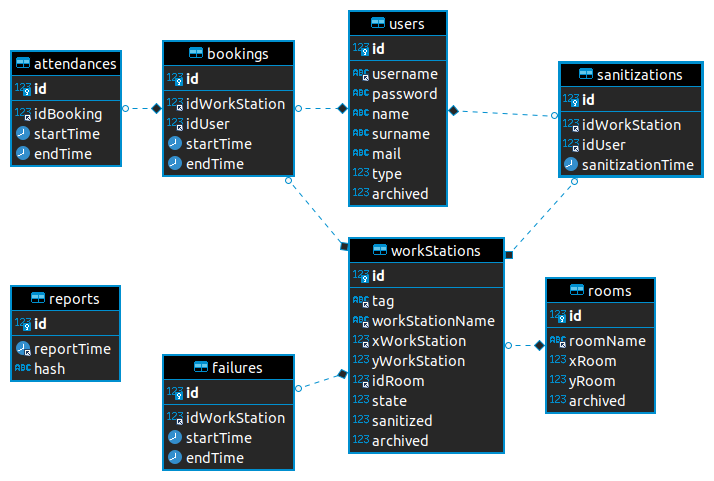
\includegraphics[width=16cm]{res/images/schemaER.png}
	\caption{Schema ER}
	\label{fig:schema ER}
\end{figure}

\subsubsection{Descrizione}
\paragraph{Attendances}
Entità che raccoglie i dati relativi alle occupazioni di una postazione. È descritta dai seguenti campi:
\begin{itemize}
	\item id: identificativo dell'occupazione;
	\item idBooking: identificativo della prenotazione a cui l'occupazione è associata;
	\item startTime: data e ora di inizio dell'occupazione;
	\item endTime: data e ora di fine dell'occupazione.
\end{itemize}

\paragraph{Bookings}
Entità che raccoglie i dati relativi alle prenotazioni di una postazione. È descritta dai seguenti campi:
\begin{itemize}
	\item id: identificativo della prenotazione;
	\item idWorkStation: identificativo della postazione prenotata;
	\item idUser: identificativo dell'utente che ha effettuato la prenotazione;
	\item startTime: data e ora di inizio della prenotazione;
	\item endTime: data e ora di fine della prenotazione;
	\item archived: segnala se la prenotazione sia stato archiviata: 0 non archiviata, 1 archiviata.
\end{itemize}

\paragraph{Users}
Entità che raccoglie i dati relativi agli utenti. È descritta dai seguenti campi:
\begin{itemize}
	\item id: identificativo dell'utente;
	\item username: nome dell'utente;
	\item password: hash della password;
	\item name: nome proprio dell'utente;
	\item surname: cognome dell'utente;
	\item mail: indirizzo e-mail dell'utente;
	\item type: tipo di utente: 0 amministratore, 1 dipendente, 2 addetto alle pulizie;
	\item archived: segnala se l'utente sia stato archiviato: 0 non archiviato, 1 archiviato.
\end{itemize}

\paragraph{Sanitizations}
Entità che raccoglie i dati relativi alle igienizzazioni. È descritta dai seguenti campi:
\begin{itemize}
	\item id: identificativo dell'igienizzazione;
	\item idWorkStation: identificativo della postazione igienizzata;
	\item idUser: identificativo dell'utente che ha effettuato l'igienizzazione;
	\item sanitizationTime: data e ora in cui è stata effettuata l'igienizzazione.
\end{itemize}

\paragraph{Reports}
Entità che raccoglie le certificazioni generate dal sistema. È descritta dai seguenti campi:
\begin{itemize}
	\item id: identificativo della certificazione;
	\item reportTime: data e ora in cui è avvenuta la certificazione;
	\item blockchainHash: indirizzo della transazione in cui il fileHash è stato salvato;
	\item fileHash: hash della certificazione.
\end{itemize}

\paragraph{workStationsFailures}
Entità che raccoglie i guasti relativi alle postazioni. È descritta dai seguenti campi:
\begin{itemize}
	\item id: identificativo del guasto;
	\item idWorkStation: identificativo della postazione soggetta a guasto;
	\item startTime: data e ora di inizio guasto;
	\item endTime: data e ora di fine guasto.
	\item archived: segnala se il guasto sia stato archiviato: 0 non archiviato, 1 archiviato.
\end{itemize}

\paragraph{roomsFailures}
Entità che descrive le stanze inaccessibili. È descritta dai seguenti campi:
\begin{itemize}
	\item id: identificativo dell'inaccessibilità;
	\item idRoom: identificativo della stanza inaccessibile;
	\item startTime: data e ora di inizio inaccessibilità;
	\item endTime: data e ora di fine inaccessibilità.
	\item archived: segnala se l'inaccessibilità sia stata archiviata: 0 non archiviata, 1 archiviata.
\end{itemize}

\paragraph{WorkStations}
Entità che raccoglie i dati relativi alle postazioni. È descritta dai seguenti campi:
\begin{itemize}
	\item id: identificativo della postazione;
	\item tag: codice esadecimale descrivente il tag NFC associato alla postazione;
	\item workStationName: nome della postazione;
	\item xWorkStation: posizione x (ascissa) in cui si trova la postazione all'interno della stanza;
	\item xWorkStation: posizione y (ordinata) in cui si trova la postazione all'interno della stanza;
	\item idRoom: identificativo della stanza in cui si trova la postazione;
	\item state: descrive lo stato in cui si trova la postazione: 0 libera, 1 occupata, 2 prenotata, 3 guasta;
	\item sanitized: descrive se la postazione è igienizzata: 0 non igienizzata, 1 igienizzata; 
	\item archived: segnala se la postazione sia stata archiviata: 0 non archiviata, 1 archiviata.
\end{itemize}

\paragraph{Rooms}
Entità che raccoglie i dati relativi alle stanze. È descritta dai seguenti campi:
\begin{itemize}
	\item id: identificativo della stanza;
	\item roomName: nome della stanza;
	\item xRoom: dimensione x (lunghezza) della stanza. Si assume che le stanze siano rettangolari;
	\item yRoom: dimensione y (larghezza) della stanza;
	\item archived: segnala se la stanza sia stata archiviata: 0 non archiviata, 1 archiviata;
	\item unavailable: segnala se la stanza sia inaccessibile: 0 accessibile, 1 non accessibile.
\end{itemize}
